\subsection*{Model Component}
The relation between the problem class and the solution class has been changed from a aggregation to a association, as a solution is not a part of a problem.

The relation between the Person class and the Department class has been changed from a composition to a aggregation, as a personon can easily exist by itself without a department, which is the case with clients. The cardinality has also been changed from 1 - 0..* to 0..1 - 0..*.

A new associative relation between the person class and a comment class has been created, which shows the relation between the author and the comment. A person can have zero to multiple comments, and a comment can only have one author.
	

\begin{figure}[p]%
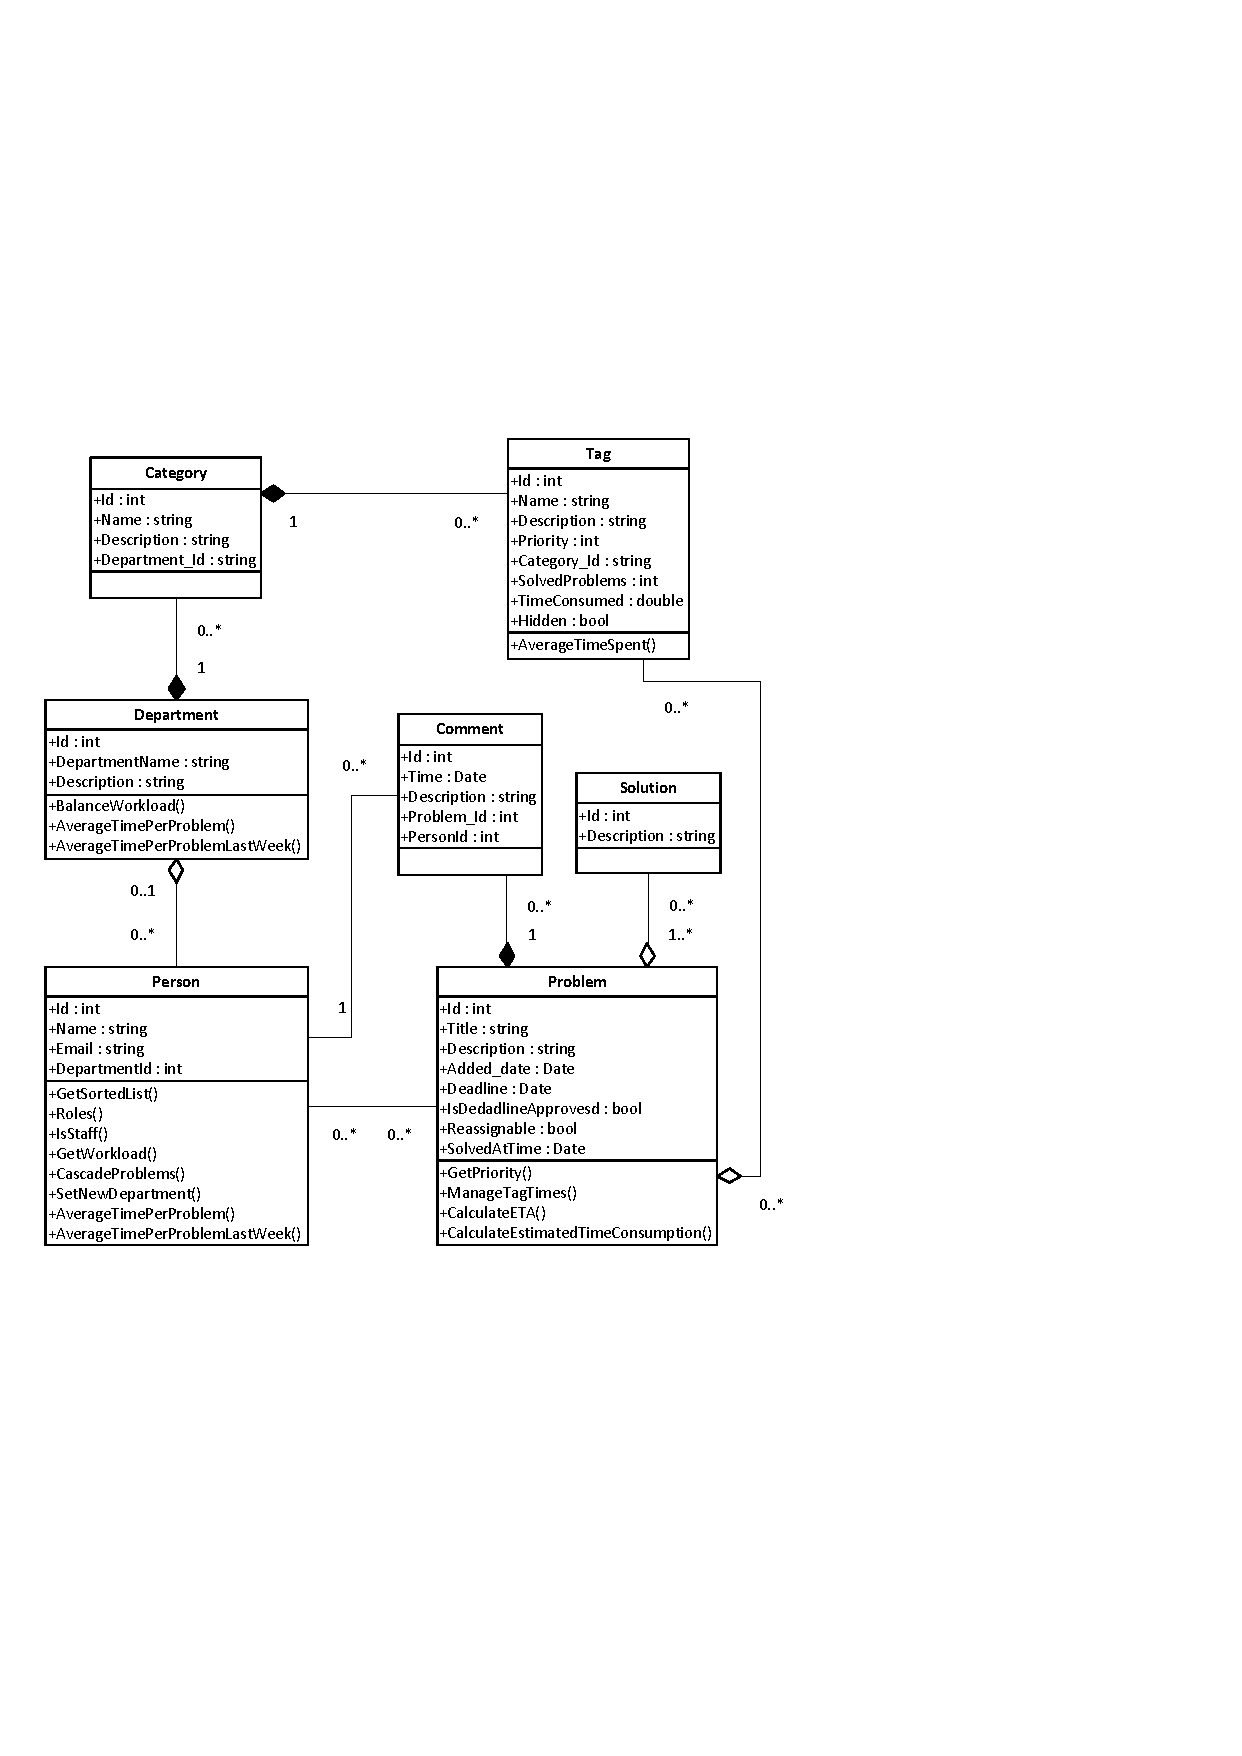
\includegraphics[clip=true, height=1.0\textwidth, trim=0.5cm 5cm 7.5cm 7cm]{ClassDiagramV3.pdf}%
\label{fig:modelcomponent}
\morscaption{The mode!!l component}
\end{figure}

